%\documentclass{exercise}
\documentclass[answers]{exercise}
%\documentclass[additions]{exercise}
%\documentclass[additions,answers]{exercise}
\usepackage{amsmath}


%%%%%%%%%%%%%%%%%%%%%%%%%%%%%%%%%%%%%%%%%%%%%%%%%%%%%%%%%%%%%%%%%%%%%%%%
\bsauthor{Granitzer}
\bsyear{2012}
\bsreadingtitle{Medientechnik}


%%%%%%%%%%%%%%%%%%%%%%%%%%%%%%%%%%%%%%%%%%%%%%%%%%%%%%%%%%%%%%%%%%%%%%%%
\begin{document}

\exerciseheader[\today]{�bungsblatt 4}

\vspace{2cm} 

\section*{Aufgaben} 

%%%%%%%% Farbmodelle %%%%


\begin{exercise}{Farbmodelle und Digitalisierung von Bildern - Allgemeine Fragen}
\label{ex-de-mt-informationstheorie-fragen}
\begin{enumerate}
\item Was sind Farbmodelle und wie stehen sie in Zusammenhang mit der menschlichen Wahrnehmung?
\item Erkl�ren Sie das CIE-XYZ Farbmodell. Welche Farben sind damit abbildbar und was spezifiziert die Black-Body Kurve?
\item Erkl�ren Sie das RGB und das CYMK Farbmodell und vergleichen sie es mit dem YCrCb/YPbPr Farbmodell.
\item Wie kann das HSV bzw. HSL Farbmodell als Zylinder dargestellt werden und worin liegt der Unterschied zum RGB Modell? 
\item Beschreiben sie den Digitalisierungsprozess bei Bildern sowie die damit verbundenen wichtigsten Kenngr��en?
\item Was bedeutet Dithering?
\item Definieren sie den Begriff Gamma-Korrektur sowie dessen Anwendungsbereich.
\item Beschreiben sie den grundlegenden Aufbau von TIFF, BMP, GIF und PNG.
\item Worin unterscheiden sich PNG und GIFs?
\item Diskutieren sie die verschiedenen Anwendungsszenarien von TIFF,
  BMP, GIF, PNG, JPEG und EXIF.
\item Erkl\"aren Sie die JPEG Kompression. Wo entstehen Verluste?
  Erkl\"aren Sie den Zusammenhang zur menschlichen Wahrnehmung.
\answer{[Siehe Vorlesungsfolien}
\end{enumerate}
\end{exercise}

 %%% Wissensfragen: TODO - Erweitern



\begin{exercise}{Farbmodelle - Umrechnung}
\label{ex-de-mt-Farbmodelle Umrechnung}

Rechnen Sie die folgenden RGB Werte in das CYM, CIE-XYZ, YUV und das YCrCb Farbsystem um:

\begin{itemize}
  \item RGB(255,255,0)
  \item RGB(0,255,0)
  \item RGB(0,0,0)
  \item RGB(92,33,28)
\end{itemize}

\answer{\url{http://start.farben.rehbein.net/} od. \url{http://www.informatics.occursus.de/hp/Farben/Java/SyncFM.htm}
od. \url{http://www.cg.info.hiroshima-cu.ac.jp/~miyazaki/knowledge/teche01.html}


Werte sind auf 0-1 normiert.
\small
\begin{tabular}{c|cccc}
  RGB             & CMY          & CIE-XYZ           &    YUV/YIQ				& YCrCb \\
  RGB(1,1,0)  & CMY(0,0,255) 		& 	XYZ(0.772,0.929,0.15)& YUV(0.886, 0.321, -0.314) & 210/255, 16/255, 146/255\\
  RGB(0,1,0) & CMY(255 ,0 ,255) 	&0.342,0.707,0.13		 & 154/255, 54/255, 34/255  \\
  RGB(0,0,0) & CMY(255,255,255) & 0,0,0 & 0,0,0 & 16/255, 128/255, 128/255\\
  RGB(0.36,0.123,0.1) & 0.638, 0.877, 0.9&0.216,0.174,0.117&0.192,0.15,0.044& 59/255, 117/255, 154/255\\
\end{tabular}
}

\end{exercise}

 %%% Farbmodelle allgemein



\begin{exercise}{CIE XYZ Farbmodell}
\label{ex-de-mt-cie}
\begin{itemize}
  \item Erkl�ren sie das CIE XYZ Farbmodell und die wichtigsten ableitbaren Punkte im CIE-XYZ Diagramm (siehe nachfolgende Abbildung).
   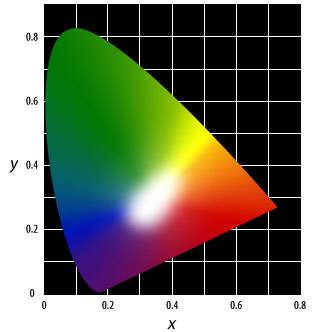
\includegraphics{figure/cie_4}
  \answer{
  \begin{itemize}
  \item Weisspunkt
  \item Black Body Curve - Farbtemperatur
  \item Spektrallinie
  \item Purpurlinie
  \item Gerade WP auf (W Weisspunkt, P Punkt auf der Spektrallinie) zeigt Farben gleicher Farbt�ne
\end{itemize}
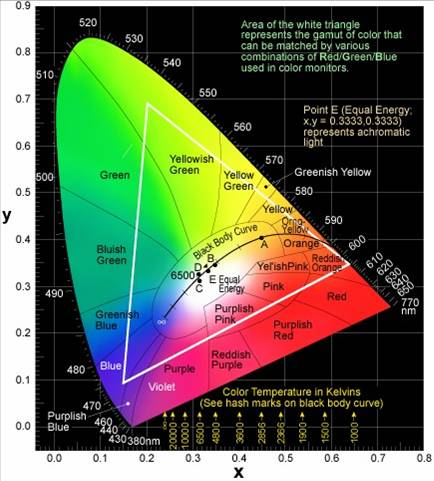
\includegraphics{figure/cie-answer-a}
  }
  \item Welchen Effekt hat ein Wei�abgleich im Diagramm?
  \answer{Er verschiebt den Weisspunkt entlang der Black Body Curve}
  \item Erkl�ren sie den Begriff Gamut und wie der RGB Gamut im CIE-XYZ Farbmodell abgebildet wird.
  \answer{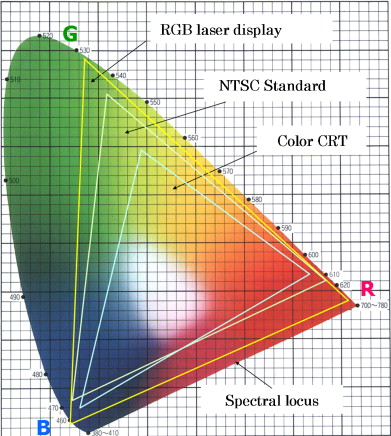
\includegraphics{figure/cie-answer-c-d}}
  \item Nehmen sie zwei RGB Quellen mit unterschiedlichem Farbbereich und unterschiedlicher Farbtemperatur an. Erkl�ren sie damit den Effekt der unterschiedlichen Farbtemperatur auf die dargestellten Farben.
  \answer{Wenn der WP verschoben ist, �ndert sich auch die Farbtonlinie und wird in der N�he von Wei� entsprechend bl�ulicher oder gelber (in Abh�ngigkeit von der Temperatur) } 
\end{itemize}

\end{exercise}

 %%% CIE Farbmodell

%

\begin{exercise}{Dithering 5 Pkt.}
\label{ex-de-mt-dithering}
Erkl�ren sie den Prozess des Dithering f�r Farb- und Grauwertbilder und implementieren sie den Floyd-Steinberg-Algorithmus in einer Programmiersprache Ihrer Wahl.\\[5ex]
\textit{Hinweis:} Diese Aufgabe dient auch als Hinweis f�r die Bewertung der Kleinprojekt und der entsprechenden Punktevergabe. Die Implementierung des Dithering Algorithmus in einem Kleinprojekt w�rde somit mit 5 Punkten bewertet werden. 


\end{exercise}

 %%% Dithering, implementierung



\begin{exercise}{Gamma Korrektur}
\label{ex-de-mt-gamma-korrektur}
Erkl�ren sie die Gamma Korrektur in der Theorie. 
Simulieren sie eine Foto�bertragungsstrecke (Kamera zum Monitor) mittels einer Bildbearbeitungssoftware (z.B. GIMP). Nehmen sie dazu ein beliebiges Bild und zeigen sie die Zust�nde zum Zeitpunkt der Aufnahme, der Abspeicherung und der Darstellung auf einen R�hrenmonitor unter folgenden Annahmen:  \\[3ex]
\begin{itemize}
  \item Das Bild wurde Gamma encodiert (mit $\gamma=1/2.2$), die Anzeige ist linear
  \item Das Bild wurde Gamma encodiert (mit $\gamma=1/2.2$), die Anzeige f�hrt eine Gamma-Korrektur mit $\gamma=2.2$ durch
  \item Das Bild wurde \textbf{nicht} Gamma encodiert, die Anzeige f�hrt eine Gamma-Korrektur mit $\gamma=2.2$ durch
  \item Das Bild wurde \textbf{nicht} Gamma encodiert, die Anzeige ist linear.
\end{itemize}
\answer{siehe \url{http://www.cambridgeincolour.com/tutorials/gamma-correction.htm}

Beispiel einer Gamma-Kurve mit unterschiedlichen Koeffizienten zur Anpassung der Grauwerte.\\

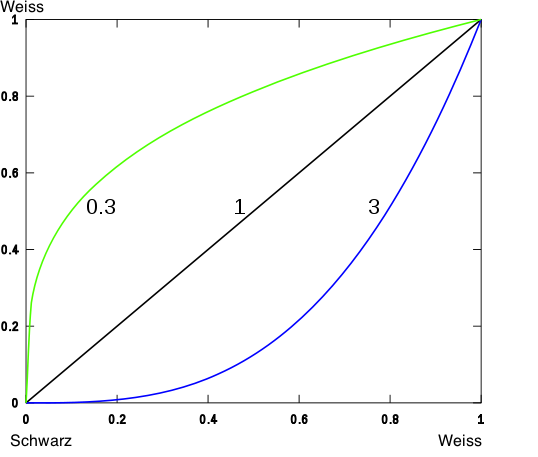
\includegraphics[width=0.5\textwidth]{figure/gamma-korrektur}\\

\textbf{Fall 1:} Ein $\gamma=1/2.2$ encodiertes Bild bedeutet, dass dunklere Pixel einen h�heren Helligkeitswert erhalten. Die Kodierung wird verwendet, um eine Ann�herung an die Wahrnehmung unserers Auges zu erreichen, welches dunkle Abstufungen besser wahrnimmt als helle.
Ist die Anzeige nun linear, werden diese Grauwerte auch so dargestellt, d.h. dunkle Grauwerte werden heller. Das Gesamtgamma des Systems entspricht $\gamma=1/2.2$\\
Rohbild (ohne Encoding): 

\includegraphics[width=\textwidth]{figure/gamma-linear}\\

Helleres Bild:

\includegraphics[width=\textwidth]{figure/gamma-0_45}


\textbf{Fall 2:} Bild Gamma encodiert, Anzeige f�hrt Gamma Korrektur durch. Das Gesamtgamma des Systems entspricht $\gamma=1$, d.h. die Gamma Kodierung wird bei der Anzeige korrigiert indem hellere Grauwerte der Gammakurve entsprechend dunkler dargestellt werden.\\ 
Rohbild (ohne Encoding)==Dargestelltes Bild: 

\includegraphics[width=\textwidth]{figure/gamma-linear}

\textbf{Fall 3:} Bild nicht Gamma encodiert, Anzeige ist Gamma korrigierend. Das Gesamtgamma des Systems entspricht $\gamma=2.2$\\
Rohbild (ohne Encoding): 

\includegraphics[width=\textwidth]{figure/gamma-linear}
Die dunklen Bereiche werden bei der Anzeige nochmals dunkler dargestellt.\\
Dargestelltes Bild:

\includegraphics[width=\textwidth]{figure/gamma-2_2}

 
\textbf{Fall 4:} Bild nicht Gamma encodiert, Anzeige f�hrt keine Gamma Korrektur durch. Das Gesamtgamma des Systems entspricht $\gamma=1$\\
Rohbild (ohne Encoding)==Dargestelltes Bild: 

\includegraphics{figure/gamma-linear}
}
\end{exercise}

 %%% Praxis Gamma Korrektur

%%%%%%%% Bildverarbeitung/JPEG %%%%


\begin{exercise}{JPEG Kompression}
\label{ex-de-mt-JPEG}
Geben Sie einen \"Uberblick \"uber die einzelne Schritte der JPEG Transformation.
\begin{itemize}
  \item Erkl�ren Sie den Schritt des Chroma-Subsampling im Detail 
  \item Erkl�ren Sie den Schritt zur Quantisierung der DCT Koeffizienten sowie die in der DCT verwendeten Basisfunktionen unter Verwendung des folgenden Demonstrators: \url{http://demonstrations.wolfram.com/JPEGCompressionAlgorithm/}
\end{itemize}

\end{exercise}

 %% JPEG Transformation - Theorie



\begin{exercise}{Histogrammmanipulationen}
\label{ex-de-mt-histogram}
Gegeben sei folgendes 3-Bit Graustufenbild:
\[
\begin{pmatrix}
	4 & 4 & 4 & 4 & 4\\
	3 & 4 & 5 & 4 & 3\\
	3 & 5 & 5 & 5 & 3\\
	3 & 4 & 5 & 4 & 3\\
	4 & 4 & 4 & 4 & 4\\
\end{pmatrix}
\]
\begin{itemize}
  \item Bilden Sie das Grauwerthistogramm.
  \item F�hren sie eine Histogrammeinebnung am obigen Graustufenbild durch. Zeigen Sie das entstehende kumulative Histogramm sowie das transformierte Bild.
  \answer{
%see digital image processing by jayaraman\\

\begin{tabular}{l|cccccccc}
Graustufen 						 & 0  & 1 & 2 & 3 & 4 & 5 & 6 & 7\\
\# Pixel (Histogram)  			 & 0  & 0 & 0 & 6 & 14 & 5 & 0 & 0\\
Kumulative Summe (kum. Hist.) 	 & 0  & 0 & 0 & 6 & 20 & 25 & 25 & 25\\
Spreizungshistogramm 
($B^{neu}(x,y)=\frac{B(x,y)-3}{2}*7$)	 & 6  & 0 & 0 & 0 & 14 & 0 & 0 & 5 \\

Neuer Grauwert bei Einebnung 
($G^{neu}(i)=\frac{7}{25}*H_{kum}(i)$) & 0  & 0 & 0 & 2 & 6 & 7 & 7 &
7 \\
%Achtung: die Zeile mit Einebnung zeigt die neuen Grauwerte!

\end{tabular}

Gespreizte Matrix:
\[
\begin{pmatrix}
	4 & 4 & 4 & 4 & 4\\
	0 & 4 & 7 & 4 & 0\\
	0 & 7 & 7 & 7 & 0\\
	0 & 4 & 7 & 4 & 0\\
	4 & 4 & 4 & 4 & 4\\
\end{pmatrix}
\]


Einebnung d. Matrix:
\[
\begin{pmatrix}
	6 & 6 & 6 & 6 & 6\\
	2 & 6 & 7 & 6 & 2\\
	2 & 7 & 7 & 7 & 2\\
	2 & 6 & 7 & 6 & 2\\
	6 & 6 & 6 & 6 & 6\\
\end{pmatrix}
\]
 }
  \item F�hren Sie eine Histogrammspreizung am obigen Graustufenbild durch.  Zeigen Sie das entstehende Histogramm sowie das transformierte Bild.
  \item Zeigen sie den Unterschied zwischen einer Histogrammspreizung (Streching) und einer Histogrammeinebnung (Equalization) mit der Bildbearbeitungssoftware GIMP.
  
 \answer{
Take image on slide Spreizung  and use GIMP Functions Color Auto Equalize and Color => Stretch Contrast and compre the Histogramm
 }  
\end{itemize}




\end{exercise}

  %% Histogrammanalyse



\begin{exercise}{Filteroperationen}
\label{ex-de-mt-filter}
Gegeben ist folgendes 8-Bit Graustufenbild:
\[
\begin{pmatrix}
	0 & 0 & 0 & 0 & 0\\
	0 & 0 & 255 & 0 & 0\\
	0 & 0 & 255 & 255 & 255\\
	0 & 0 & 255 & 255 & 255\\
	0 & 0 & 255 & 255 & 255\\
\end{pmatrix}
\]


\answer{
Als Bild: 

\includegraphics[width=.1\textwidth]{figure/binary-image-2}
}


Wenden sie folgende Filter auf dieses Bild an:
\begin{itemize}
  \item $3\times 3$ Medianfilter
  
  
  \answer{
  \[
\begin{pmatrix}
	0 & 0 & 0 & 0 & 0\\
	0 & 0 & \mathbf{0} & 0 & 0\\
	0 & 0 & 255 & 255 & 255\\
	0 & 0 & 255 & 255 & 255\\
	0 & 0 & 255 & 255 & 255\\
\end{pmatrix}
\]
Als Bild:\\

\includegraphics[width=.1\textwidth]{figure/binary-image-median}
  }
  
  \item $3\times 3$- Boost Filter
  
    \answer{
 
 
 
    Boost-Filter:\\
    \[
    B^{neu}(x,y) = \begin{pmatrix}
    -1  & -1 & -1 \\
    -1 & 9   & -1 \\
    -1  & -1  & -1 \\
    \end{pmatrix}
    * N_8(x,y)
    \] 
    Bild nach Anwendung:
     \[
\begin{pmatrix}
	0 & -255   & -255  & -255   & 0\\
	0 & -2*255 & 7*255 & -4*255 & -3*255\\
	0 & -3*255 & 5*255 & 3*255 & 4*255\\
	0 & -3*255 & 4*255 & 255 & 255\\
	0 & -3*255 & 4*255 & 255 & 255\\
\end{pmatrix}
\]
Die Werte sind au�erhalb des darstellbaren Bereichs. Es gibt zwei M�glichkeiten damit umzugehen:
\begin{itemize}
  \item Clipping:


\[
 B(x,y) = \begin{cases}
        0  & B(x,y)<0 \\
        255  & B(x,y)>255 \\
        B(x,y)  & sonst
        \end{cases}
\]

  \item Skalierung $B(x,y)=\frac{B(x,y)-B_{min}}{B_{max}-B_{min}}$
\end{itemize}
Unter Anwendung von Clipping ergibt sich:
  \[
\begin{pmatrix}
	0 & 0 & 0 & 0 & 0\\
	0 & 0 & 255 & 0 & 0\\
	0 & 0 & 255 & 255 & 255\\
	0 & 0 & 255 & 255 & 255\\
	0 & 0 & 255 & 255 & 255\\
\end{pmatrix}
\]

 }
  \item $3\times 3$- Laplace Filter (ohne 45� Geradendetektion, d.h. 4er Nachberschaft)
  
  \answer{
  Laplace-Filter:\\
    \[
    B^{neu}(x,y) = \begin{pmatrix}
    0  & -1 & 0 \\
    -1 & 4   & -1 \\
    0  & -1  & 0 \\
    \end{pmatrix}
    * N_8(x,y)
    \] 
    Bild nach Anwendung:
     \[
\begin{pmatrix}
	0 & 0    & -255  &  0     & 0\\
	0 & -255 & 3*255 & -2*255 & -255\\
	0 & -255 & 255   & 255    & 255\\
	0 & -255 & 255   & 0      & 0\\
	0 & -255 & 255   & 0      & 0\\
\end{pmatrix}
\]
Die Werte sind au�erhalb des darstellbaren Bereichs
Unter Anwendung von Clipping ergibt sich:
  \[
\begin{pmatrix}
	0 & 0 & 0 & 0 & 0\\
	0 & 0 & 255 & 0 & 0\\
	0 & 0 & 255 & 255 & 255\\
	0 & 0 & 255 & 0 & 0\\
	0 & 0 & 255 & 0 & 0\\
\end{pmatrix}
\]
Als Bild:\\


\includegraphics[width=.1\textwidth]{figure/binary-image-laplace}
  }
  \item $3\times 3$- Gaussfilter
   \answer{
  Gau�-Filter:\\
    \[
    B^{neu}(x,y) = 1/16*\begin{pmatrix}
    1 & 2 & 1 \\
    2 & 4 & 2 \\
    1  & 2  & 1 \\
    \end{pmatrix}
    * N_8(x,y)
    \] 
    Bild nach Anwendung:
     \[
\begin{pmatrix}
	0 & 255/16   & 2/16*255   & 1/16*255 & 0\\
	0 & 3/16*255 & 7/16*255   & 6/16*255 & 0\\
	0 & 4/16*255 & 11/16*255  & 13/16*255   & 12/16*255\\
	0 & 4/16*255 & 12/16*255  & 16/16*255   & 16/16*255\\
	0 & 4/16*255 & 12/16*255  & 16/16*255   & 16/16*255\\
\end{pmatrix}
\]
Als Bild:

\includegraphics[width=.1\textwidth]{figure/binary-image-gauss}
  }
  \item (Optional, 1-Pkt.) Verwenden Sie ein beliebiges RGB Bild um in der Bildbearbeitungssoftware GIMP den Effekt der oben genannten Filter zu zeigen (Men�punkt Filter, Generic, Convolution Matrix). Erl�utern Sie die Effekte der Normalisierung sowie der Offset Funktion. 
\end{itemize}

Hinweis: Setzen sie das Bild an den R�ndern einfach fort

\end{exercise}

  %% Filter

\end{document} 
 

%%%%%%%%%%%%%%%%%%%%%%%%%%%%%%%%%%%%%%%%%%%%%%%%%%%%%%%%%%%%%%%%%%%%%%%%
 